% Options for packages loaded elsewhere
\PassOptionsToPackage{unicode}{hyperref}
\PassOptionsToPackage{hyphens}{url}
%
\documentclass[
]{article}
\usepackage{amsmath,amssymb}
\usepackage{iftex}
\ifPDFTeX
  \usepackage[T1]{fontenc}
  \usepackage[utf8]{inputenc}
  \usepackage{textcomp} % provide euro and other symbols
\else % if luatex or xetex
  \usepackage{unicode-math} % this also loads fontspec
  \defaultfontfeatures{Scale=MatchLowercase}
  \defaultfontfeatures[\rmfamily]{Ligatures=TeX,Scale=1}
\fi
\usepackage{lmodern}
\ifPDFTeX\else
  % xetex/luatex font selection
\fi
% Use upquote if available, for straight quotes in verbatim environments
\IfFileExists{upquote.sty}{\usepackage{upquote}}{}
\IfFileExists{microtype.sty}{% use microtype if available
  \usepackage[]{microtype}
  \UseMicrotypeSet[protrusion]{basicmath} % disable protrusion for tt fonts
}{}
\makeatletter
\@ifundefined{KOMAClassName}{% if non-KOMA class
  \IfFileExists{parskip.sty}{%
    \usepackage{parskip}
  }{% else
    \setlength{\parindent}{0pt}
    \setlength{\parskip}{6pt plus 2pt minus 1pt}}
}{% if KOMA class
  \KOMAoptions{parskip=half}}
\makeatother
\usepackage{xcolor}
\usepackage[margin=1in]{geometry}
\usepackage{longtable,booktabs,array}
\usepackage{calc} % for calculating minipage widths
% Correct order of tables after \paragraph or \subparagraph
\usepackage{etoolbox}
\makeatletter
\patchcmd\longtable{\par}{\if@noskipsec\mbox{}\fi\par}{}{}
\makeatother
% Allow footnotes in longtable head/foot
\IfFileExists{footnotehyper.sty}{\usepackage{footnotehyper}}{\usepackage{footnote}}
\makesavenoteenv{longtable}
\usepackage{graphicx}
\makeatletter
\def\maxwidth{\ifdim\Gin@nat@width>\linewidth\linewidth\else\Gin@nat@width\fi}
\def\maxheight{\ifdim\Gin@nat@height>\textheight\textheight\else\Gin@nat@height\fi}
\makeatother
% Scale images if necessary, so that they will not overflow the page
% margins by default, and it is still possible to overwrite the defaults
% using explicit options in \includegraphics[width, height, ...]{}
\setkeys{Gin}{width=\maxwidth,height=\maxheight,keepaspectratio}
% Set default figure placement to htbp
\makeatletter
\def\fps@figure{htbp}
\makeatother
\setlength{\emergencystretch}{3em} % prevent overfull lines
\providecommand{\tightlist}{%
  \setlength{\itemsep}{0pt}\setlength{\parskip}{0pt}}
\setcounter{secnumdepth}{-\maxdimen} % remove section numbering
\ifLuaTeX
\usepackage[bidi=basic]{babel}
\else
\usepackage[bidi=default]{babel}
\fi
\babelprovide[main,import]{spanish}
% get rid of language-specific shorthands (see #6817):
\let\LanguageShortHands\languageshorthands
\def\languageshorthands#1{}
\ifLuaTeX
  \usepackage{selnolig}  % disable illegal ligatures
\fi
\usepackage{bookmark}
\IfFileExists{xurl.sty}{\usepackage{xurl}}{} % add URL line breaks if available
\urlstyle{same}
\hypersetup{
  pdftitle={Práctica 2: Arquitectura y prototipo funcional del proyecto},
  pdfauthor={Azul Noguera; Patricio Guledjian; Rocio Gonzalez Cingolani; Vincent Jasou; Gabriel Zamy},
  pdflang={es-ES},
  hidelinks,
  pdfcreator={LaTeX via pandoc}}

\title{Práctica 2: Arquitectura y prototipo funcional del proyecto}
\usepackage{etoolbox}
\makeatletter
\providecommand{\subtitle}[1]{% add subtitle to \maketitle
  \apptocmd{\@title}{\par {\large #1 \par}}{}{}
}
\makeatother
\subtitle{Link al repositorio:
\url{https://github.com/azulnogueraa/Proyecto_AW}}
\author{Azul Noguera \and Patricio Guledjian \and Rocio Gonzalez
Cingolani \and Vincent Jasou \and Gabriel Zamy}
\date{2024-04-14}

\begin{document}
\maketitle

{
\setcounter{tocdepth}{3}
\tableofcontents
}
\newpage

\section*{Memoria de la estructura del proyecto}

\subsection{Introducción}\label{introducciuxf3n}

Learnique se presenta como una innovadora plataforma de educación en
línea diseñada para transformar el panorama actual del aprendizaje
digital. Distinguiéndose por su enfoque en la personalización, Learnique
no solo ofrece acceso a una amplia gama de recursos educativos, sino que
también adapta la experiencia de aprendizaje a las necesidades
individuales de cada usuario. A través de la implementación de
tecnologías avanzadas, Learnique busca optimizar la retención de
información y maximizar la satisfacción del estudiante, ofreciendo una
solución integral que va más allá de la mera transmisión de
conocimientos teóricos. Esta plataforma es el resultado de un meticuloso
análisis de las limitaciones presentes en los modelos educativos en
línea convencionales, marcando el comienzo de una era donde el
aprendizaje digital es genuinamente inclusivo, accesible y efectivo para
todos.

\subsubsection{Tipos de Usuarios}\label{tipos-de-usuarios}

Learnique atiende a una diversidad de usuarios, cada uno con distintas
metas y necesidades educativas. A continuación, se describen los
principales tipos de usuarios y las funcionalidades específicas
diseñadas para cada grupo:

\begin{itemize}
\item
  Estudiantes: Individuos que buscan expandir su conocimiento y
  habilidades en áreas específicas. Estos usuarios pueden acceder a
  cursos personalizados que se ajustan a su nivel de experiencia y ritmo
  de aprendizaje.
\item
  Educadores: Profesores y formadores que buscan complementar su
  material didáctico con recursos interactivos y actualizados. La
  plataforma permite a los educadores enriquecer su enseñanza con
  contenido diverso y herramientas de valuación avanzadas.
\item
  Administradores: Responsables de gestionar y supervisar la plataforma,
  asegurando que el contenido sea relevante, actualizado y de alta
  calidad. Los administradores también juegan un papel crucial en la
  moderación de la comunidad de usuarios, la implementación de mejoras
  basadas en la retroalimentación y el mantenimiento de la
  infraestructura técnica de Learnique.
\end{itemize}

\newpage

\subsection{Listado de scripts para las
vistas}\label{listado-de-scripts-para-las-vistas}

\subsubsection{Pagina Principal}\label{pagina-principal}

\begin{itemize}
\tightlist
\item
  index.php : Pantalla principal de la página web.
\end{itemize}

\subsubsection{Comun}\label{comun}

\begin{itemize}
\item
  topBar.php : Cabecera de la web
\item
  curso.php : Vista de un curso en particular.
\end{itemize}

\subsubsection{Plantilla}\label{plantilla}

\begin{itemize}
\tightlist
\item
  plantilla.php : Plantilla que será llamada por todas las vistas.
\end{itemize}

\subsubsection{F1: Gestión de Roles: Estudiante, Profesor,
Administrador}\label{f1-gestiuxf3n-de-roles-estudiante-profesor-administrador}

\begin{itemize}
\item
  login.php : Pantalla de login
\item
  registro.php : Pantalla de registro
\item
  logout.php : Pantalla de logout
\end{itemize}

\subsubsection{F2: Gestión de Inscripciones y
Matriculaciones}\label{f2-gestiuxf3n-de-inscripciones-y-matriculaciones}

\begin{itemize}
\item
  inscripcion.php : Pantalla de inscripción a un curso (se agrega el
  curso al carrito)
\item
  carrito.php : Pantalla de carrito de compras
\end{itemize}

\subsubsection{F3: Gestión de Búsqueda con
Filtros}\label{f3-gestiuxf3n-de-buxfasqueda-con-filtros}

\begin{itemize}
\item
  cursos.php : Pantalla de listado de cursos. A partir de ahí, podemos
  seleccionar el curso para acceder a la información que deseamos.

  \begin{itemize}
  \item
    trading.php : vista de el curso de trading
  \item
    blockchain.php : vista de el curso de blockchain
  \item
    cripto.php : vista de el curso de criptomonedas
  \item
    marketing.php : vista de el curso de marketing
  \end{itemize}
\end{itemize}

(estos cuatros cursos son ejemplos para entender lo que queremos hacer
despues con la base de datos.)

\begin{itemize}
\item
  curso.php : vista para un curso en particular, va a reemplazar los 4
  previos.
\item
  buscar\_cursos.php : Buscador de cursos.
\end{itemize}

\subsubsection{F4: Panel de
Administración}\label{f4-panel-de-administraciuxf3n}

\begin{itemize}
\tightlist
\item
  ajustes.php : En ajustes se podrá borrar usuarios y administrar
  cursos.
\end{itemize}

\subsubsection{F5: Gestión de Comunicación: Estudiantes y
Profesores}\label{f5-gestiuxf3n-de-comunicaciuxf3n-estudiantes-y-profesores}

\begin{itemize}
\tightlist
\item
  chat.php : Pantalla de chat
\end{itemize}

\vspace{12mm}

\subsection{Listado de scripts
adicionales}\label{listado-de-scripts-adicionales}

\begin{itemize}
\item
  Clase de identidad de las tablas de la base de datos:

  \begin{itemize}
  \item
    Admin.php
  \item
    Estudiante.php
  \item
    Profesor.php
  \item
    Registrado.php
  \item
    Curso.php
  \end{itemize}
\item
  Reorganización de la funcionalidad asociada a la gestión de los
  usuarios:

  \begin{itemize}
  \tightlist
  \item
    Usuario.php
  \end{itemize}
\item
  Centralización de la gestión de conexiones a bases de datos y otras
  operaciones de la aplicación.

  \begin{itemize}
  \tightlist
  \item
    Aplicacion.php:
  \end{itemize}
\item
  Reorganización de la gestión de formularios:

  \begin{itemize}
  \item
    Formulario.php
  \item
    FormurioInscripcion.php
  \item
    FormularioLogin.php
  \item
    FormularioRegistro.php
  \end{itemize}
\item
  Configuración e inicialización de la aplicación:

  \begin{itemize}
  \tightlist
  \item
    Config.php
  \end{itemize}
\item
  buscador.php
\end{itemize}

\newpage

\subsection{Estructura de la base de
datos}\label{estructura-de-la-base-de-datos}

\begin{figure}
\centering
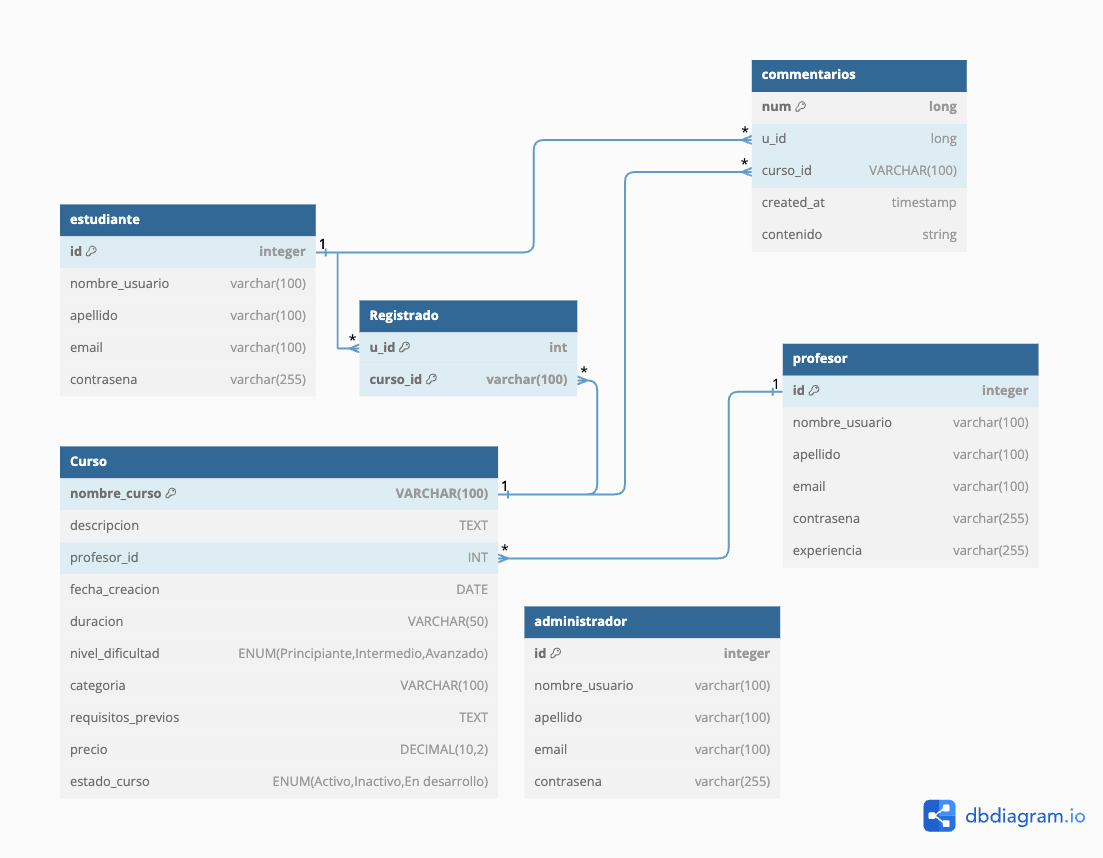
\includegraphics[width=0.85\textwidth,height=\textheight]{../img/diagrama.png}
\caption{Diagrama de la estructura de la base de datos}
\end{figure}

La arquitectura de nuestra base de datos está meticulosamente diseñada
para sustentar una plataforma educativa online que ofrece una
experiencia integral tanto para estudiantes como para profesores. El
diagrama adjunto proporciona una representación visual de las relaciones
y los campos clave de la base de datos.

La tabla \texttt{estudiante} almacena los datos esenciales del usuario,
incluyendo un identificador único \texttt{id}, el
\texttt{nombre\_usuario}, \texttt{apellido}, \texttt{email}, y una
\texttt{contraseña} segura. Esta tabla es fundamental para la gestión de
cuentas y la personalización de la experiencia del usuario.

Paralelamente, la tabla \texttt{profesor} captura información detallada
de los educadores en la plataforma, como sus credenciales de acceso,
\texttt{experiencia} profesional y especializaciones. El vínculo entre
los cursos y los profesores se establece mediante un campo de clave
foránea \texttt{profesor\_id} que conecta con el identificador único del
profesor.

Los cursos se detallan en la tabla \texttt{curso}, que incluye un nombre
descriptivo, \texttt{nombre\_curso}, una \texttt{descripcion} extensa
del contenido, \texttt{fecha\_creacion}, \texttt{duracion} estimada, y
un \texttt{nivel\_dificultad} que clasifica el curso. Además, cada curso
tiene asignado una \texttt{categoria}, \texttt{requisitos\_previos}
necesarios para el alumno y un \texttt{precio}, además de un estado
(\texttt{estado\_curso}) que indica si está activo, inactivo o en
desarrollo.

Para gestionar las inscripciones, disponemos de la tabla
\texttt{Registrado}, que establece una relación entre los estudiantes y
los cursos a los que se han inscrito, mediante los campos \texttt{u\_id}
y \texttt{curso\_id}. Esta tabla es crucial para el seguimiento de las
inscripciones activas y el acceso a los contenidos del curso.

Por último, la tabla \texttt{comentarios} permite a los estudiantes y
profesores interactuar y discutir dentro del contexto de un curso,
facilitando el intercambio de conocimientos y opiniones. Registra el
\texttt{u\_id} y \texttt{curso\_id} correspondiente, junto con la
\texttt{fecha} del comentario y su \texttt{contenido}.

\newpage

\subsection{Prototipo funcional del
proyecto}\label{prototipo-funcional-del-proyecto}

\subsubsection{Profesores:}\label{profesores}

\begin{longtable}[]{@{}
  >{\raggedright\arraybackslash}p{(\columnwidth - 8\tabcolsep) * \real{0.2346}}
  >{\raggedright\arraybackslash}p{(\columnwidth - 8\tabcolsep) * \real{0.1235}}
  >{\raggedright\arraybackslash}p{(\columnwidth - 8\tabcolsep) * \real{0.3333}}
  >{\raggedright\arraybackslash}p{(\columnwidth - 8\tabcolsep) * \real{0.1481}}
  >{\raggedright\arraybackslash}p{(\columnwidth - 8\tabcolsep) * \real{0.1605}}@{}}
\toprule\noalign{}
\begin{minipage}[b]{\linewidth}\raggedright
nombre de usuario
\end{minipage} & \begin{minipage}[b]{\linewidth}\raggedright
apellido
\end{minipage} & \begin{minipage}[b]{\linewidth}\raggedright
email
\end{minipage} & \begin{minipage}[b]{\linewidth}\raggedright
contraseña
\end{minipage} & \begin{minipage}[b]{\linewidth}\raggedright
experiencia
\end{minipage} \\
\midrule\noalign{}
\endhead
\bottomrule\noalign{}
\endlastfoot
javier & bravo &
\href{mailto:javier@learnique.edu}{\nolinkurl{javier@learnique.edu}} &
javier1 & alta \\
eva & ullan &
\href{mailto:eva@learnique.edu}{\nolinkurl{eva@learnique.edu}} & eva12 &
alta \\
\end{longtable}

\subsubsection{Estudiantes:}\label{estudiantes}

\begin{longtable}[]{@{}
  >{\raggedright\arraybackslash}p{(\columnwidth - 6\tabcolsep) * \real{0.2794}}
  >{\raggedright\arraybackslash}p{(\columnwidth - 6\tabcolsep) * \real{0.1471}}
  >{\raggedright\arraybackslash}p{(\columnwidth - 6\tabcolsep) * \real{0.3971}}
  >{\raggedright\arraybackslash}p{(\columnwidth - 6\tabcolsep) * \real{0.1765}}@{}}
\toprule\noalign{}
\begin{minipage}[b]{\linewidth}\raggedright
nombre de usuario
\end{minipage} & \begin{minipage}[b]{\linewidth}\raggedright
apellido
\end{minipage} & \begin{minipage}[b]{\linewidth}\raggedright
email
\end{minipage} & \begin{minipage}[b]{\linewidth}\raggedright
contraseña
\end{minipage} \\
\midrule\noalign{}
\endhead
\bottomrule\noalign{}
\endlastfoot
azul & noguera &
\href{mailto:azul@learnique.edu}{\nolinkurl{azul@learnique.edu}} &
azul1 \\
rocio & gonzalez &
\href{mailto:rocio@learnique.edu}{\nolinkurl{rocio@learnique.edu}} &
rocio1 \\
patricio & guledjian &
\href{mailto:patricio@learnique.edu}{\nolinkurl{patricio@learnique.edu}}
& patricio1 \\
gabriel & zamy &
\href{mailto:gabriel@learnique.edu}{\nolinkurl{gabriel@learnique.edu}} &
gabriel1 \\
vincent & jansou &
\href{mailto:vincent@learnique.edu}{\nolinkurl{vincent@learnique.edu}} &
vincent1 \\
\end{longtable}

\subsubsection{Administradores:}\label{administradores}

\begin{longtable}[]{@{}
  >{\raggedright\arraybackslash}p{(\columnwidth - 6\tabcolsep) * \real{0.2794}}
  >{\raggedright\arraybackslash}p{(\columnwidth - 6\tabcolsep) * \real{0.1471}}
  >{\raggedright\arraybackslash}p{(\columnwidth - 6\tabcolsep) * \real{0.3971}}
  >{\raggedright\arraybackslash}p{(\columnwidth - 6\tabcolsep) * \real{0.1765}}@{}}
\toprule\noalign{}
\begin{minipage}[b]{\linewidth}\raggedright
nombre de usuario
\end{minipage} & \begin{minipage}[b]{\linewidth}\raggedright
apellido
\end{minipage} & \begin{minipage}[b]{\linewidth}\raggedright
email
\end{minipage} & \begin{minipage}[b]{\linewidth}\raggedright
contraseña
\end{minipage} \\
\midrule\noalign{}
\endhead
\bottomrule\noalign{}
\endlastfoot
admin & admin &
\href{mailto:admin@learnique.edu}{\nolinkurl{admin@learnique.edu}} &
admin1 \\
\end{longtable}

\newpage

\subsection{VPS}\label{vps}

\vspace{5mm}

URL al servicio de Guacamole:

\url{https://vm013.containers.fdi.ucm.es/p3_g2/}

\begin{itemize}
\item
  Usuario: vm013
\item
  Contraseña: UEp7y90WZsGqKUtAG\_J8
\end{itemize}

\newpage

\subsection{Actividades de los
integrantes}\label{actividades-de-los-integrantes}

\subsubsection{Azul Noguera}\label{azul-noguera}

\begin{itemize}
\tightlist
\item
  Style.css
\item
  index.php estructura
\item
  Creación de la memoria
\item
  Ordenamiento de las carpetas y los ficheros
\item
  Contribución en carpeta mysql
\item
  Contribución a diagrama de estructura de base de datos
\end{itemize}

\subsubsection{Rocio Gonzalez}\label{rocio-gonzalez}

\begin{itemize}
\tightlist
\item
  leeme.txt
\item
  Contribución en registro de usuarios
\item
  Contribución a carpeta mysql
\item
  Contribución a gestión de busqueda de cursos
\item
  Contribución a panel de administración
\item
  Contribución a la gestión de inscripciones y matriculación
\end{itemize}

\subsubsection{Patricio Guledjian}\label{patricio-guledjian}

\begin{itemize}
\tightlist
\item
  Contribución a gestión de busqueda de cursos
\item
  Contribución a panel de administración
\item
  Contribución al style.css
\item
  Contribución en la carpeta mysql
\end{itemize}

\subsubsection{Vincent Jasou}\label{vincent-jasou}

\begin{itemize}
\tightlist
\item
  Validación de ficheros php
\item
  Contribución a registro de usuarios
\item
  Reorganización del codigo en clases
\item
  Contribución a gestión de busqueda de cursos
\item
  Contribución a panel de administración
\end{itemize}

\subsubsection{Gabriel Zamy}\label{gabriel-zamy}

\begin{itemize}
\tightlist
\item
  Contribución a diagrama de estructura de base de datos
\item
  Contribución en carpeta mysql
\item
  Reorganización del codigo en clases
\item
  Contribución a la gestión de inscripciones y matriculación
\end{itemize}

\end{document}
